%-------------------------
% Resume in Latex
% Author : Harshibar
% Based off of: https://github.com/jakeryang/resume
% License : MIT
%------------------------

\documentclass[letterpaper,11pt]{article}

\usepackage{latexsym}
\usepackage[empty]{fullpage}
\usepackage{titlesec}
\usepackage{marvosym}
\usepackage[usenames,dvipsnames]{color}
\usepackage{verbatim}
\usepackage{enumitem}
\usepackage[hidelinks]{hyperref}
\usepackage{fancyhdr}
\usepackage[english]{babel}
\usepackage{tabularx}
\usepackage{xcolor}
\usepackage[style=apa, backend=biber]{biblatex}
\usepackage{tikz}
    \usetikzlibrary{mindmap, positioning}
% only for pdflatex
% \input{glyphtounicode}

% fontawesome
\usepackage{fontawesome5}

% fixed width
\usepackage[scale=0.95,lf]{FiraMono}

% light-grey
\definecolor{light-grey}{gray}{0.83}
\definecolor{dark-grey}{gray}{0.3}
\definecolor{text-grey}{gray}{.08}
\definecolor{teal}{HTML}{008080}
\definecolor{turquoise}{HTML}{40E0D0}


\DeclareRobustCommand{\ebseries}{\fontseries{eb}\selectfont}
\DeclareTextFontCommand{\texteb}{\ebseries}

% custom underilne
\usepackage{contour}
\usepackage[normalem]{ulem}
\renewcommand{\ULdepth}{1.5pt}
\contourlength{0.8pt}

\newcommand{\myuline}[1]{%
  \uline{\phantom{#1}}%
  \llap{\contour{white}{#1}}%
}

\newcommand{\MYhref}[2]{
\myuline{\href{#1}{{#2}}}
}%

% \def\adcv@resumeofkey{'s Résumé}
% \newcommand*{\adcvname}[2]{\def\adcv@firstname{#1}\def\adcv@lastname{#2}}
% \newcommand*{\adcvtitle}[1]{\def\adcv@title{#1}}
% \adcvname{Vsevolod}{Suschevskiy}

\newcommand{\firstname}{Vsevolod}
\newcommand{\lastname}{Suschevskiy}

\hypersetup{%
    % urlbordercolor = black,
    % pdfborderstyle={/S/U/W 1},
    pdfauthor={\firstname~\lastname},%
    pdfsubject={\firstname~\lastname's Résumé},%
    pdftitle={\firstname~\lastname's Résumé}%
      }

% custom font: helvetica-style
\usepackage{tgheros}
\renewcommand*\familydefault{\sfdefault} 
%% Only if the base font of the document is to be sans serif
\usepackage[T1]{fontenc}


\pagestyle{fancy}
\fancyhf{} % clear all header and footer fields
\fancyfoot{}
\renewcommand{\headrulewidth}{0pt}
\renewcommand{\footrulewidth}{0pt}

% Adjust margins
\addtolength{\oddsidemargin}{0in}
\addtolength{\evensidemargin}{1.5in}
\addtolength{\textwidth}{-0.05in}
\addtolength{\topmargin}{-.5in}
\addtolength{\textheight}{1.0in}
\setlist{leftmargin=0.15in, rightmargin=.5in}
\titlespacing* % starred version: first paragraph is not indented
    {\section} % <command>
    {1em} % <left>
    {3.5ex plus 1ex minus .2ex} % <before-sep>
    {2.3ex plus .2ex} % <after-sep>

\urlstyle{same}

\raggedbottom
\raggedright
\setlength{\tabcolsep}{0in}

% Sections formatting - serif
% \titleformat{\section}{
%   \vspace{2pt} \scshape \raggedright\large % header section
% }{}{0em}{}[\color{black} \titlerule \vspace{-5pt}]

% TODO EBSERIES
% sans serif sections
\titleformat {\section}{
    % \bfseries 
    \vspace{2pt}\hspace{-1pt} \raggedright \large  % header section
}{}{0em}{}[\color{teal} {\titlerule[1pt ]} \vspace{-4pt}]

% only for pdflatex
% Ensure that generate pdf is machine readable/ATS parsable
% \pdfgentounicode=1

%-------------------------
% Custom commands
\newcommand{\resumeItem}[1]{
  \item\small{
    {#1 \vspace{-1pt}}
  }
}

\newcommand{\resumeSubheading}[4]{
  \vspace{-10pt}\item
    \begin{tabular*}{\textwidth}[t]{l@{\extracolsep{\fill}}r}
      \textbf{#1} & {\color{dark-grey}\small #2}\vspace{1pt}\\ % top row of resume entry
      \hspace{2pt}\textit{#3} & {\color{dark-grey} \small #4}\\ % second row of resume entry
    \end{tabular*}\vspace{-4pt}
}

\newcommand{\resumeSubSubheading}[2]{
    \item
    \begin{tabular*}{\textwidth}{l@{\extracolsep{\fill}}r}
      \textit{\small#1} & \textit{\small #2} \\
    \end{tabular*}\vspace{-7pt}
}

\newcommand{\resumeProjectHeading}[2]{
    \item
    \begin{tabular*}{\textwidth}[t]{l@{\extracolsep{\fill}}r}
    \textbf{#1} & {\color{dark-grey}\small #2}\vspace{1pt}\\ % top row of resume entry
    \end{tabular*}\vspace{-4pt}
}

\newcommand{\resumeSubItem}[1]{\resumeItem{#1}\vspace{-4pt}}

\renewcommand\labelitemii{$\vcenter{\hbox{\tiny$\bullet$}}$}

% CHANGED default leftmargin  0.15 in
\newcommand{\resumeSubHeadingListStart}{\begin{itemize}[leftmargin=0in, label={}]}
\newcommand{\resumeSubHeadingListEnd}{\end{itemize}}
\newcommand{\resumeItemListStart}{\begin{itemize}[label={-}]}
\newcommand{\resumeItemListEnd}{\end{itemize}\vspace{0pt}}

\color{text-grey}


% publications?
\addbibresource{publications.bib}
%-------------------------------------------
%%%%%%  RESUME STARTS HERE  %%%%%%%%%%%%%%%%%%%%%%%%%%%%

\begin{document}
%----------HEADING----------
\setlength{\belowcaptionskip}{-10pt}
\vspace{-5pt}
\begin{center}
    % \textbf{\Huge Vsevolod Suschevskiy} \\ \vspace{5pt}
    % \begin{figure}[h]
  \centering
  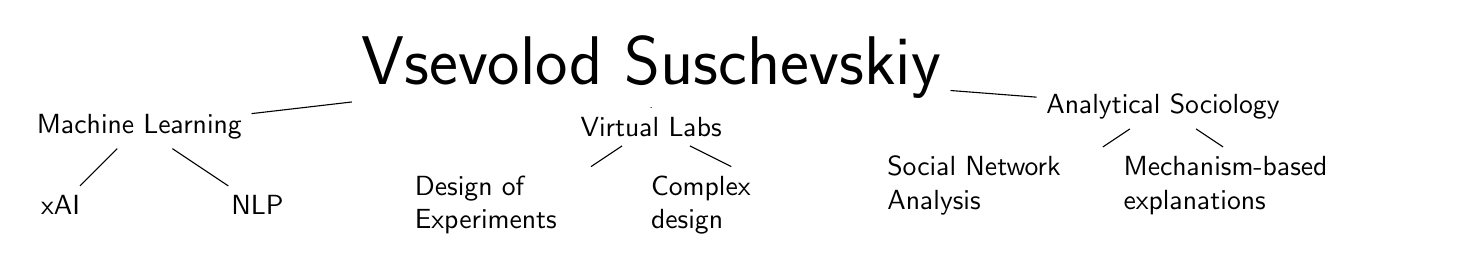
\begin{tikzpicture}[]
  \path (0,0) node (x) {\Huge{Vsevolod Suschevskiy}}
        (6.5,-0.5) node (y) {Analytical Sociology}
            (5, -1.5) node[text width=4cm] (y1) {Social Network \\ 
            Analysis}
            (8, -1.5) node[text width=4cm] (y2) {Mechanism-based \\ explanations}
        (-6.5,-0.75) node (z) {Machine Learning}
            (-7.5, -1.75) node (z1) {xAI}
            (-5, -1.75) node (z2) {NLP}
        (0,-0.75) node (k) {Virtual Labs}
            (-1.5, -1.75) node[text width=3cm] (k1) {Design of \\ Experiments}
            (2, -1.75) node[text width=4cm] (k2) {Complex \\ design};

  \draw[]   (x) -- (y)
                (y) -- (y1)
                (y) -- (y2)
            (x) -- (z)
                (z) -- (z1)
                (z) -- (z2)
            (x) -- (k)
                (k) -- (k1)
                (k) -- (k2);
\end{tikzpicture}
  % \caption{Cognitive Map of Computational Social Science Experiments}
  % \label{fig:cognitive-map}
% \end{figure}
\vspace{-5pt}
    % \vspace{-10pt}
    % \small \faPhone* \texttt{555.555.5555} \hspace{1pt} $|$
    \hspace{1pt} \texttt{vvseva@u.northwestern.edu} \hspace{1pt} $|$ 
     \hspace{1pt}  \hspace{2pt} \texttt{\MYhref{https://vvseva.quarto.pub}{vvseva.quarto.pub}} \hspace{1pt} $|$ 
    % \hspace{1pt} \faYoutube \hspace{2pt} \texttt{harshibar} \hspace{1pt} $|$
    \hspace{1pt}  \hspace{2pt}\texttt{Evanston, IL, USA}
    \\ \vspace{-1pt}
    \vspace{-5pt}
\end{center}

%------MINDMAP--------





%-----------EXPERIENCE-----------
\section{Research and Professional Experience}\label{sec:research}

  \resumeSubHeadingListStart
      \resumeSubheading
      {\MYhref{https://sonic.northwestern.edu/}{SONIC lab} at Northwestern University}{June 2022 - present}
      {Graduate Research Assistant}{Evanston, IL}
      \resumeItemListStart
        \resumeItem{Advisor: Noshir Contractor}
        \resumeItem{Data-Driven research of Human-AI Communication in teams, using multilayer-ERGMs (paper in progress)}
        \resumeItem{Designing Transition from Wizard of OZ style experiment to a digital experiment powered by LLMs and deployed on Empirica.ly platform (MVP ready)}
         \resumeItem{Interactive survey to study unfriending at Facebook (pre-pilot)}
         \resumeItem{Grant proposal writing}
         \resumeItem{Undergraduate interns supervision}
      \resumeItemListEnd

    \resumeSubheading
      {\MYhref{https://atlas.northwestern.edu/}{ATLAS lab} at Northwestern University}{Mar. - Aug. 2023}
      {Graduate Research Assistant}{Evanston, IL}
      \resumeItemListStart
        \resumeItem{Advisor: Leslie DeChurch}
        \resumeItem{Designing virtual lab experiment for studying collaboration in Human-AI teams}
      \resumeItemListEnd
      
    \resumeSubheading
      {Northwestern University}{Mar. 2023 - Aug. 2024}
      {Graduate Teaching Assistant}{Evanston, IL}
      \resumeItemListStart
        \resumeItem{Spring 2023, Spring 2024; MSC 492: Leading \& Leveraging Networks; 50+ graduate students; Prof.: Noshir Contractor}
        \resumeItem{Fall 2023 COMP SCI 330: Human-Computer Interaction; 200+ undergraduate students; lo-fi paper prototyping; Figma; Prof.: Matthew Kay}
        \resumeItem{Spring 2024, COMP SCI 341: Social Network Analysis; 75+ STEM and non-STEM students; Prof.: Noshir Contractor}
      \resumeItemListEnd 


    \resumeSubheading
      {\MYhref{https://vk.com/about\#}{Core Analytics} at VK}{July - Sep. 2021}
      {Research Internship}{St. Petersburg, Russia}
      \resumeItemListStart
        \resumeItem{Population Scale Social Network Analysis: Validating Robin Dunbar's concept of social circles on dyadic interactions, examining dynamics of social circles. Privacy-focused design recommendations.}
        \resumeItem{\MYhref{https://youtu.be/eoHZliaLYGY}{VK Teach Talk video (in Russian)}}
      \resumeItemListEnd 
      
    \resumeSubheading
      {\MYhref{https://slate.uib.no}{SLATE} Center at University of Bergen}{Jan. 2020 -- Jun. 2021}
      {Research Assistant}{Bergen, Norway}
      \resumeItemListStart
        \resumeItem{Supervisor: Dr. Mohammad Khalil}
        \resumeItem{Created a \textbf{course recommendation system} for exchange students, using Shiny, Elasticsearch, and TensorFlow.}
        \resumeItem{10+ Think aloud interviews, 50+ user test participants}
    \resumeItemListEnd

    \resumeSubheading
      {HSE University}{Sept. 2020 -- Jun. 2022}
      {Lecturer}{St.Petersburg, Russia}
      \resumeItemListStart
        \resumeItem{Data Science Minor: CS0 and CS1 for non-STEM majors; tidyverse, tidymodels, shiny; offline to online transition}
        \resumeItem{MSc UX Analytics and Information System Design: Research Seminar; Into to experiments in HCI}
        \resumeItem{MSc Data Analytics for Politics and Society: 15+ graduate students; sklearn, pandas, crowdsourcing}
      \resumeItemListEnd
    \resumeSubheading
      {European University At St. Petersburg}{Mar. -- Jun. 2022}
      {Lecturer}{St.Petersburg, Russia}
      \resumeItemListStart
        \resumeItem{Data Visualization: MSc Applied Data Analysis (PANDAN); Grammar of Graphics, ggplot2, tableau; 20+ professional and graduate students}
      \resumeItemListEnd

    \resumeSubheading
    {\MYhref{https://spb.hse.ru/en/fmcs/math/sociocomp/}{SocComp} research group at HSE University}{2017--2018; 2019--2020}
    {Junior member}{St.Petersburg, Russia}
        \resumeItemListStart
        \resumeItem{Supervisor: Prof. Alena Suvorova}
        \resumeItem{Tutorials for junior students on Bayesian network analysis and xAI, and model interpretation for Data Science minor}
        \resumeItem{Supervisor: Ilya Musabirov}
        \resumeItem{Social Network Analysis of eSports transfers in Dota 2 with ERGMs}
        \resumeItemListEnd

        \resumeSubheading
    {HSE University}{2017 Sep. -- Jun. 2020}
    {Teaching Assistant}{St.Petersburg, Russia}
        \resumeItemListStart
        \resumeItem{Data Science minor: tutorial, grading}
        \resumeItem{Theory Construction and Model Building: Undergraduate elective for Sociology Major students; Integration of theoretical frameworks, e.g. Desire-belief-opportunity, Theory of Planned behavior, Bounded rationality with Computational representation, e.g. production rules,  probabilistic models; NetLogo.}
        \resumeItemListEnd


  \resumeSubHeadingListEnd


%-----------EDUCATION-----------
\section {Education}
  \resumeSubHeadingListStart
    \resumeSubheading
      {Northwestern University}{June 2022 -- present}
      {PhD Student in Technology and Social Behavior}{Evanston, IL, USA}
    \resumeItemListStart
    \resumeItem {Advisor: Noshir Contractor}
    \resumeItem {Dissertation TBA}
        \resumeItemListEnd


    \resumeSubheading
    {HSE University}{Sept. 2020 --  Jun. 2022}
    {MSc Information Systems and Human-Computer Interaction}{St.Petersburg, Russia}
        \resumeItemListStart
        \resumeItem{Advisor: Ilya Musabirov, Alena Suvorova}
        \resumeItem{Dissertation: "Experiments in Designing Personalized Motivational Systems" is a set of virtual labs designed to test the idea of self-nudging in crowdsource workers settings}
        \resumeItemListEnd

        \resumeSubheading
    {University of Bergen}{Aug. -- Dec. 2019}
    {Exchange term}{Bergen, Norway}
        \resumeItemListStart
        \resumeItem{Research Topics in Technology Enhanced Learning; Knowledge Representation and Reasoning}
        \resumeItemListEnd  

        \resumeSubheading
    {HSE University}{Jan. 2017 --  Jun. 2020}
    {BA Sociology and Social Informatics}{St.Petersburg, Russia}
        \resumeItemListStart
        \resumeItem{Advisor: Ilya Musabirov}
        \resumeItem{Dissertation: "Computational Modelling Frameworks in Sociology: Scientometric Analysis" is a sociology of science work on how researchers transfer their epistemic beliefs from the original discipline into applied theoretical frameworks and computational representations}
        \resumeItemListEnd  

                \resumeSubheading
    {Immanuel Kant Baltic Federal University}{Sep. -- Dec. 2016}
    {Sociology}{Kaliningrad, Russia}
        \resumeItemListStart
        \resumeItem{State-funded place, but transferred after the first semester}
        \resumeItemListEnd 
        
  \resumeSubHeadingListEnd

% %-----------PROJECTS-----------

% \section{PROJECTS}
%     \resumeSubHeadingListStart
%       \resumeProjectHeading
%           {\textbf{Hyku Consulting}} {Sept. 2019 -- Mar. 2021}
%           \resumeItemListStart
%             \resumeItem{Mentored 15 students towards acceptance at top US boarding schools; achieved \textbf{100\% success rate}}
%             \resumeItem{Designed a \textbf{collaborative learning ecosystem} for students and parents with Trello, Miro, and Google Suite}
%           \resumeItemListEnd
          
%         \resumeProjectHeading
%           {\textbf{Minimal Icon Pack}}{Sept. 2020 -- Nov. 2020}
%           \resumeItemListStart
%             \resumeItem{Designed and released 100+ minimal iOS and Android icons from scratch using Procreate and Figma}
%             \resumeItem{Marketed the product and design process on {\MYhref{https://www.youtube.com/watch?v=Ju32r7QJCzk}{YouTube}}; accumulated over \textbf{\$250 in sales} on {\MYhref{https://gumroad.com/l/icons-by-harshibar}{Gumroad}}}
%           \resumeItemListEnd
          
%       \resumeProjectHeading
%          {\textbf{CommonIntern}}{Sept. 2019 -- May 2020}
%           \resumeItemListStart
%             \resumeItem{Built a Python script to automatically apply to jobs on Glassdoor using BeautifulSoup and Selenium}
%             \resumeItem{\textbf{500 stars on \MYhref{https://github.com/harshibar/common-intern}{GitHub}}; featured on {\MYhref{https://hackaday.com/2020/05/30/job-application-script-automates-the-boring-stuff-with-python}{Hackaday}}; made the front page of {\MYhref {https://www.reddit.com/r/Python/comments/gpaegj/i_was_tired_of_opening_100s_of_tabs_for/?utm_source=share}{r/python}} and {\MYhref {https://www.reddit.com/r/programming/comments/dcmbzx/i_was_tired_of_opening_100s_of_tabs_for/}{r/programming}}}
%           \resumeItemListEnd
          
%     \resumeSubHeadingListEnd


\section{Volunteer Experience}
    \resumeSubHeadingListStart
      \resumeProjectHeading
        {HELPDESK.MEDIA} {Sept. 2022} 
          \resumeItemListStart
            \resumeItem{Provided consultations on how to safely escape areas affected by war.}
          \resumeItemListEnd
        \resumeProjectHeading
        {Women Data Leaders in Russia} {Sept. 2018 -- Jun. 2020}
          \resumeItemListStart
            \resumeItem{Organized poster session; Interviewed Jana Diesner and Milena Tsvetkova; Edited video for youtube channel}
          \resumeItemListEnd
    \resumeSubHeadingListEnd

%
%-----------PROGRAMMING SKILLS-----------
\section{Skills}
 \begin{itemize}[leftmargin=0in, label={}]
    \small{\item{
     \textbf{Data analysis} {: R (\textbf{tidyverse}, igraph, rvest, bnlearn, ERGM); Python (pandas, pyspark, networkx)} \vspace{2pt} \\
    \textbf{Machine Learning} {: R (\textbf{tidymodels}, rpart, LDA, STM); Python (Tensorflow, spacy, gensim, huggingface, LLMs)} \vspace{2pt} \\
    \textbf{Visualization} {: R (ggplot2, visNetwork, plotly, shinydashboard), Tableau;  Python (Seaborn, Plotly) } \vspace{2pt} \\
    \textbf{Interactive web apps} {: R (Shiny), JavaScript (empirica.ly)} \vspace{2pt} \\
    \textbf{Data Bases} {: SQL (ClickHouse, MongoDB), noSQL (Elasticsearch)} \vspace{2pt} \\
    \textbf{All other random stuff} {: Linux, AWS, git, NetLogo, Prolog, Open Broadcast Software, Adobe Premiere Pro, \LaTeX}
    }}
 \end{itemize}

 %-----------Awards-----------
\section{Awards}
 \begin{itemize}[leftmargin=0in, label={}]
    \small{\item{
     \textbf{Toloka Research Grant (Yandex LLC)} {: Supported my MSc thesis experimental research on behavioural nudges and boosts. Feb 2022.} \vspace{2pt} \\
    }}
    \small{\item{
     \textbf{Peter and Adrienne Barris Outstanding Teaching Assistant} {: Northwestern Computer Science honors and recognizes students who demonstrate excellence in computer science mentoring and teaching. Spring 2024 Social Network Analysis class. (COMP-SCI 341)} \vspace{2pt} \\
    }}
 \end{itemize}

 %-----------Languages-----------
\section{Languages}
 \begin{itemize}[leftmargin=0in, label={}]
    \small{\item{
     \textbf{Russian} {: Native} \vspace{2pt} \\
     \textbf{English} {: C1/C2} \vspace{2pt} \\
     \textbf{French} {: beginner} \vspace{2pt} \\
    }}
 \end{itemize}


%---------------PUBLICATIONS----------------------------
\defbibfilter{papers}{
  type=article or
  type=inproceedings or 
  type=inbook
}
\newrefcontext[labelprefix=P, sorting=ydnt]

\nocite{suschevskiy_creating_2021}
\nocite{musabirov_teaching_2020}
\nocite{marchenko_analysis_2018}
\nocite{suschevskiy_network_2018}

\printbibliography[filter=papers,title={Publications}]

%---------------presentations----------------------------
\defbibfilter{presentations}{
  type=misc 
}
\newrefcontext[labelprefix=C, sorting=ydnt]

\nocite{CODE2023}
\nocite{IC2S22023}
\nocite{HCID2022}
\nocite{Sunbelt2020}
\nocite{SIGCSE2020}
\nocite{ICCSS2019}


\printbibliography[filter=presentations,title={Conference presentations}]



\end{document}
